\begin{bibunit}[IEEEtran.bst]

\chapter*{Introduction}
\addcontentsline{toc}{chapter}{Introduction}
\chaptermark{Introduction}

Understanding and anticipating the ramifications of climate change represents a pressing challenge of our era.
Enhancing our knowledge of Earth's systems is a key factor in confronting this challenge.
  Given that the primary source of factual information about the Earth system is observational data, improving our ability to exploit these data could lead to better monitoring and understanding of our planet.
  This thesis focus on the development of methods to exploit satellite observations for improving our knowledge of ocean surface dynamics. 
  More specifically we're asking how advances in deep learning research can be beneficial to ocean observation analysis.
  
  In order to introduce the potentials of deep learning for tackling ocean observation problems, we'll introduce the necessary methodological components involved when addressing an observation problem by walking through the development of a thermometer graduation procedure. This simplified problem will help illustrate and contextualize the complementary roles of data and domain knowledge when addressing this class of problem and naturally invite deep learning components in certain aspects of the resolution. 

  This will first consist in decomposing the process of mapping the level of the thermometer to the temperature. Then we'll look at the challenges met when evaluating a graduated thermometer. We'll consider the different sources of errors before finally formalizing the necessary components for developing a thermometer graduation procedure.


  \section{Intro}
 When  one is interested in knowing the temperature, we observe the level of a thermometer.
As such observations are the proxy by which we know about the quantities that are of interest to us. 
  The development of methods to exploit observations to know about geophysical quantities of interest (QoI) is the core subject of this manuscript. 
  In order to introduce the necessary concepts to contextualize this manuscript, we'll walk through the development of a thermometer calibration procedure.
  The first step will be to explicit the process of mapping the level of the thermometer to the temperature.
  Then we'll look at the challenges met when evaluating a calibrated thermometer.
  We'll consider the different sources of errors before finally formalizing the necessary components for developing a thermometer calibration procedure.

  This will introduce the challenges brought by observation problems as well as the different approaches to facing them.

  We will then present the specific usecases addressed in this document detail how our contributions address the challenges.

  Once the necessary concepts have been introduced, we'll present how tools brought by deep learning research can contribute to this resolution process and the challenges specific to observation tasks that we can anticipate.

  Finally we'll describe our contributions with the specific observation use-case and the learning-related challenge addressed. 
  
  \section{Graduating a thermometer}
\subsection{Mapping observations to quantity of interest}
\begin{figure}[h]
    \centering
        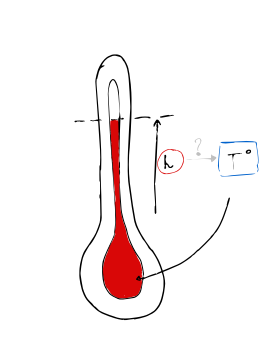
\includegraphics[clip, width=3cm]{Introduction/pics/therm_pb.png}
    \caption{Thermometer Graduation problem illustration. Given a simple liquid based thermometer, we aim at finding the matching between height of the liquid within the glass tube and temperature.}
    \label{fig:therm_calib}
\end{figure}

Let's consider a standard liquid based thermometer that consists of a liquid in a glass tube .
When interested in knowing the temperature, we observe the level of a thermometer.
In order to do so, someone had to graduate the thermometer. 
This seemingly simple action can be detailed in a two-step process, which involves the construction of a theoretical model and its calibration using real-world data.

The first step involves compiling theories and assumptions to construct a model linking the observed level and the actual temperature.
For instance, based on our knowledge of fluid dilation in response to temperature, assuming the diameter of the tube is constant with height, we can posit that the level is linearly correlated with the temperature.
This model introduces two parameters: the slope and offset of our linear model that need to be ascertained.

The second step involves determining these parameters. This step requires some calibration data as inputs. They are traditionally obtained by immersing the thermometer in icing and boiling water to acquire the levels corresponding to 0°C and 100°C.
  Using those data points, a linear system can then be used to solve for the parameters. Which finally gives use our level-to-temperature mapping


The solution, therefore, is a product of both theory and data, and can be reduced to two key components: the model and the calibration algorithm.

Interestingly, the model's complexity can often be inversely proportional to the amount of data required. For instance, a model with fewer assumptions demands more data. If we were to abandon the assumption of the thermometer tube's constant diameter, we would need to incorporate a parameterization of the tube diameter in our model. This addition creates more parameters and consequently demands additional data for calibration.

Conversely, having access to more data can allow us to work with fewer assumptions. Suppose we possess a well-calibrated thermometer that can provide unlimited data points. In that case, we could reduce our assumptions to a minimum and rely heavily on empirical evidence, marking each thermometer graduation using data directly from our well-calibrated thermometer.

With these carefully calibrated graduations now etched onto our thermometer, we can use the liquid level as a convenient stand-in for the temperature. However, an important question remains: How can we verify the accuracy of our newly calibrated thermometer?

\begin{figure}[h]
\centering
\begin{tabular}{ccc}

    Step 1: 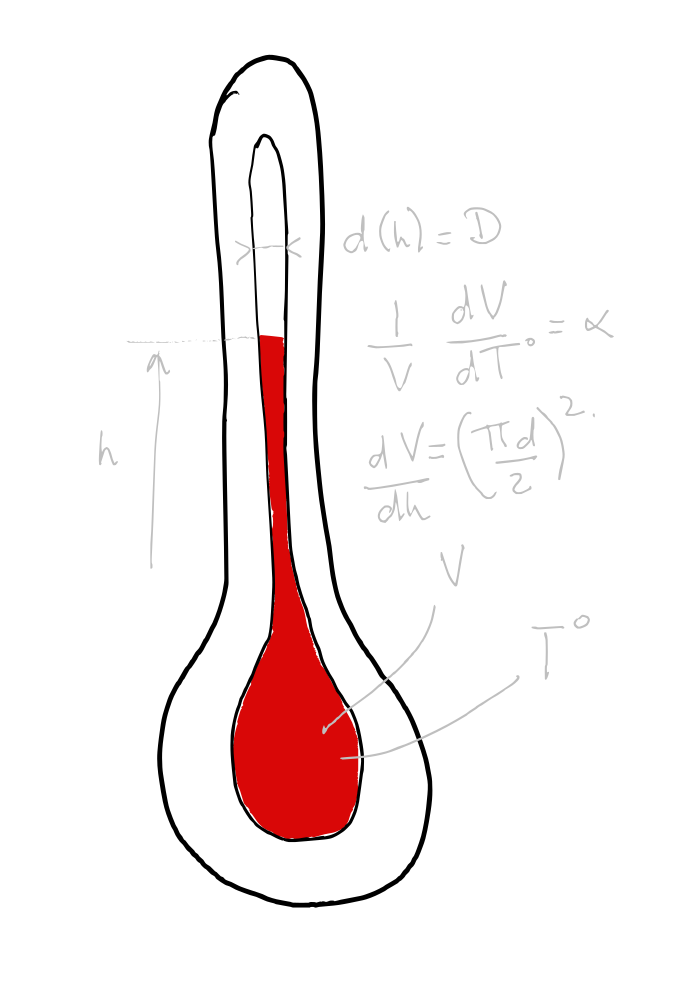
\includegraphics[clip, width=3cm, width=3cm]{Introduction/pics/therm_theroy.png} &    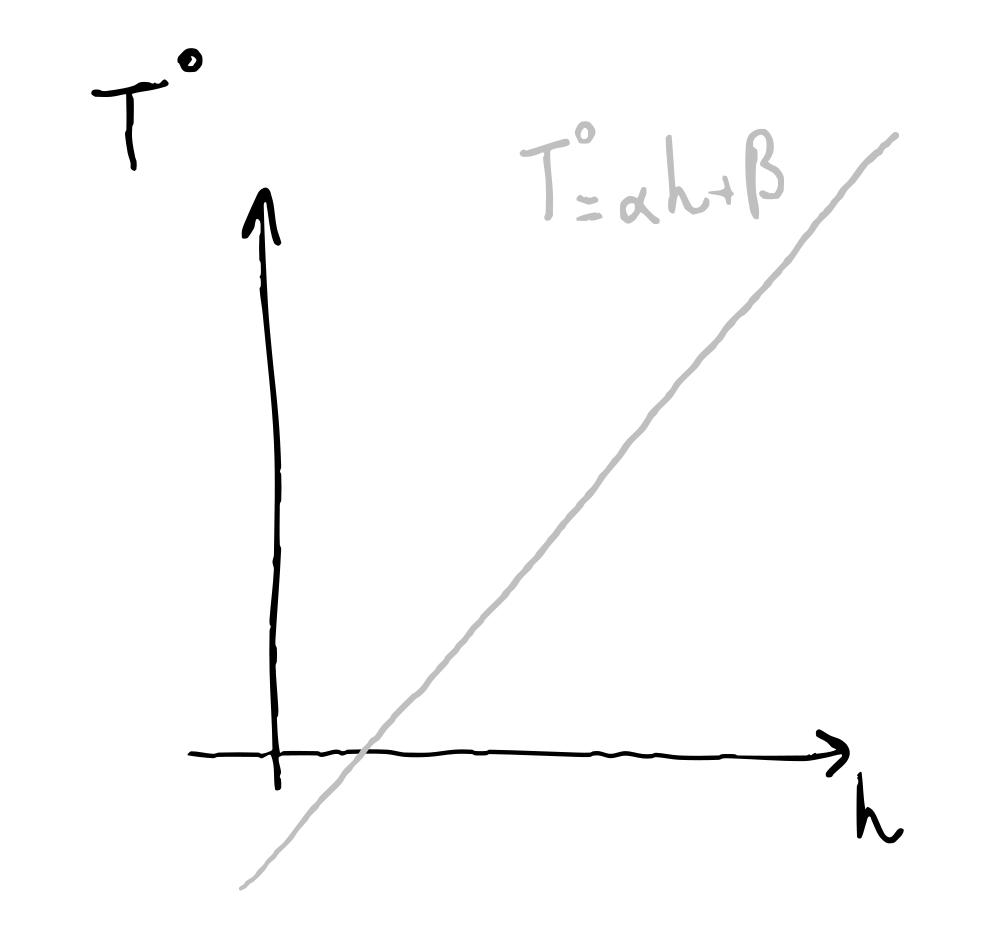
\includegraphics[clip, width=5cm]{Introduction/pics/therm_model.png}     \\  
     Step 2: 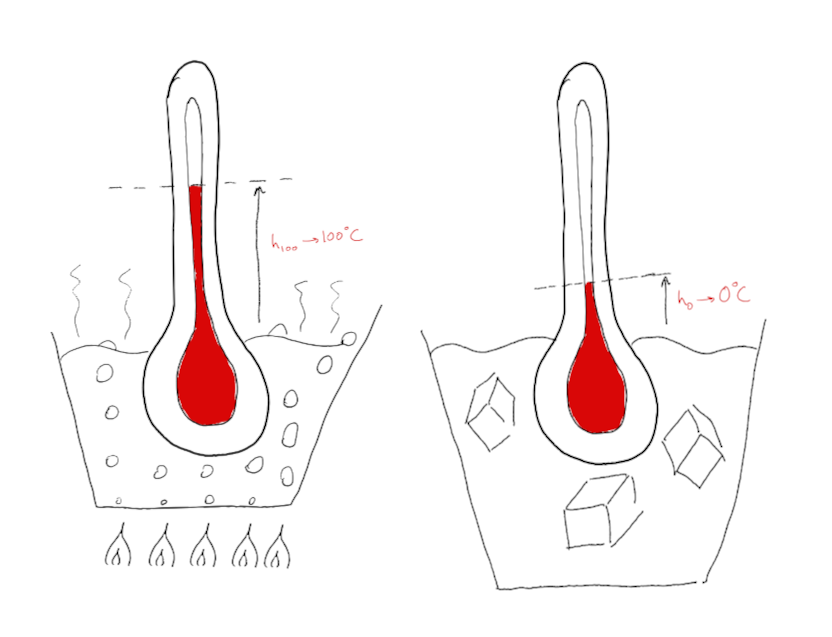
\includegraphics[clip, width=4cm, height=4cm, trim={2cm 1cm 2cm 2cm}]{Introduction/pics/therm_obs.png} &    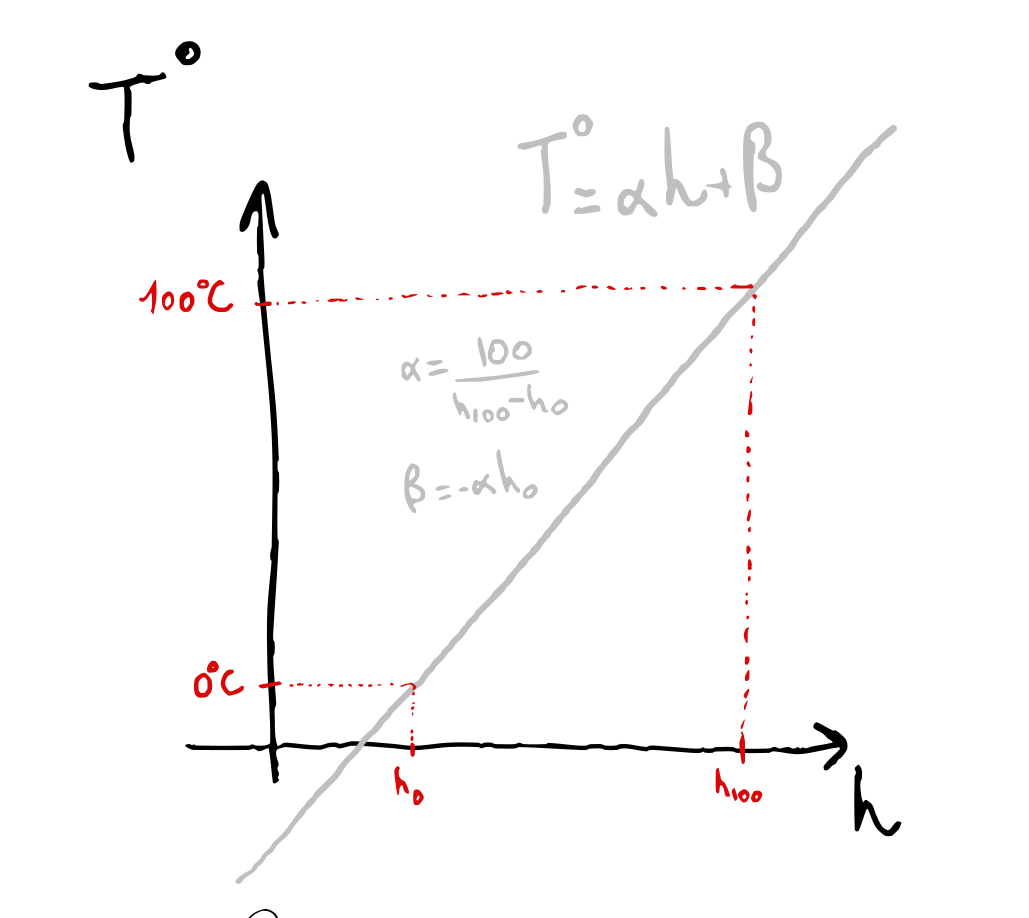
\includegraphics[clip, width=5cm]{Introduction/pics/therm_calib.png}     \\  
\end{tabular}

    \caption{Mapping thermometer level to temperature. The first step consists in compiling theoritical knowledge to determine a model of the level to temperature relationship. This model define the set of candidate graduations. The second step consists in leveraging data to chose the best candidate graduation through some calibration procedure.}
    \label{fig:therm_mapping}
\end{figure}

\subsection{Evaluation}

Without evaluation the use of our calibrated instrument would solely rely in the faith given to our mapping above.
Being novice calibrators, we need to quantify the thermometers quality through metrics.

In our case the most intuitive metric for characterizing our thermometer's quality is be the precision of the graduations.
Note that some situations may put importance on other characteristic such at the range at which it's functional.
  In order to properly evaluate our calibrated instrument, we need to test it in conditions corresponding to its intended use. (testing it domestic thermometer 5 kilometers underwater would not give relevant evaluation).

 To do so, let's explicit some assumptions made on what we expect from our thermometer.
  For example that it needs to "be accurate to the half of degree", "have response time under 10 minutes", "work between -30°C and 200°C" "work at a reasonable atmospheric pressure" etc...

Then we need data to measure the precision of our thermometer in a way that is representative of how we want our thermometer to behave. Using a trustworthy reference like a third-party well-graduated thermometer, we could compare the measurements of the reference with the one given by our solution.
  An example evaluation procedure could be to confront the measurements of the two instruments at different temperatures such as: in a freezer, in a fridge, at ambiant room temperature and in an oven.

Using the procedure above, we can compute our precision metrics and assess if the quality of our graduated thermometer is acceptable.
This exercise, raises some critical points about evaluation. The process relies on two components that require a deep understanding of the thermometer's intended use: a suitable choice of metric and representative data. If the chosen metrics don't align with the intended use of the thermometer, the evaluation will be flawed. Similarly, if the data isn't representative of the thermometer's intended use, the evaluation will also be flawed.
 Furthermore, the reliability of the reference thermometer is pivotal. If the reference thermometer is not well-graduated, the best of metrics won't be able to correctly evaluate our thermometer. 

It's also crucial to differentiate between calibration data, which is used to generate a solution, and evaluation data, which is used to assess the solution's quality.
A well-functioning thermometer should provide accurate temperature readings even for levels it wasn't calibrated on. Also, evaluation data should differ from calibration data. If we only measure precision at 0°C and 100°C, a thermometer that perfectly fits the calibration data would receive the highest metric, even if the other graduations were nonsensical.

\begin{figure}
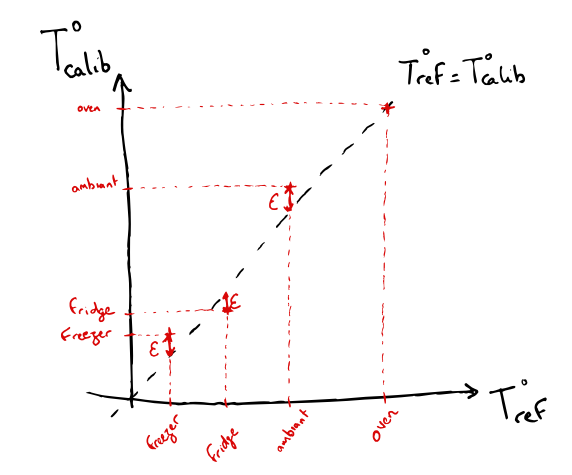
\includegraphics[clip, width=6cm]{Introduction/pics/errors.png}  
    \centering
    \caption{Evaluation and errors. Given some evaluation data and choice of metric, we can compute the errors associated with our graduation. $T_{calib}$ and $T_{ref}$ are respectively the temperatures given by our graduation and a reference well graduated thermometer}
    \label{fig:err_sources}
\end{figure}



 \subsection{Sources of errors}

Given an evaluation procedure, the errors are the gap to the reference and can be attributed to three sources.

\begin{figure}
\begin{tabular}{c |c|c}

     \hspace{-.15\linewidth}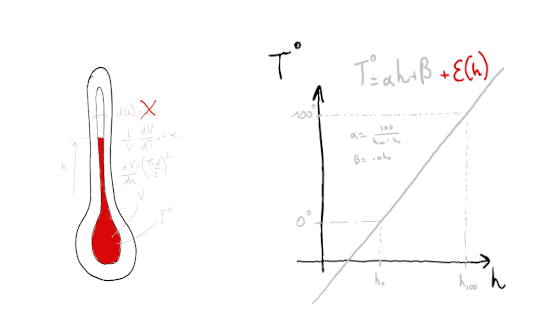
\includegraphics[width=.4\linewidth]{Introduction/pics/model_err_w_source.png}  &
     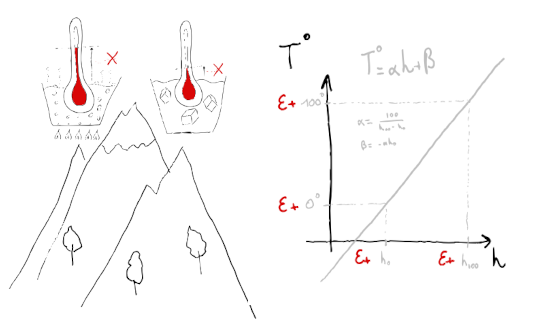
\includegraphics[width=.4\linewidth]{Introduction/pics/data_err_w_source.png} &
     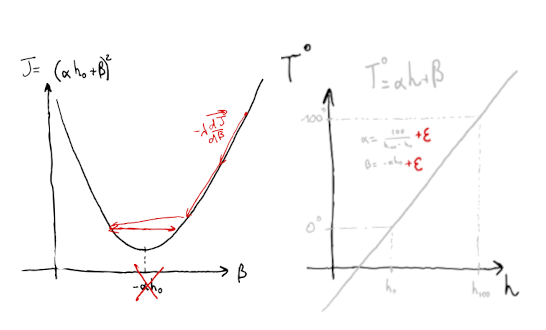
\includegraphics[width=.4\linewidth]{Introduction/pics/optim_err_w_source.png} \\
     \hspace{-.15\linewidth}Model &  Data &  Algorithm \\
\end{tabular}
    \centering
    \caption{Illustration of the different sources of errors for the thermometer graduation. From left to right: model errors result from erroneous assumptions about the system. Data errors result from inaccuracies in the calibration data and algorithmic errors result from a failure of the calibration procedure to select the best candidate from the model.}
    \label{fig:err_sources}
\end{figure}
 The model is a source of error if the assumptions made were inaccurate. For example if the diameter of the tube is not constant with height the linear correlation between level and temperature is not exact and will induce errors when interpreting the level.

 Even with perfect assumptions, noisy data can introduce errors in the calibration. If we interpreted our 0°C and 100°C in icing and boiling water at the top of a mountain with lower atmospheric pressure, we will have calibrated our parameters with erroneous measurements and the subsequent graduation of our thermometer will be inaccurate.

 Finally even with perfect assumption and perfect data, the algorithm used to find the solution's parameters can be a source of errors if it fails to find the optimal parameters. For example if we solve for the parameters with a gradient descent method, using a step size too big will prevent finding the exact parameters which will also results errors in the subsequent measurements.

In order to develop a graduation procedure, we need to take those sources of error into account. The graduation procedure choice will not only depend on the level-temperature relationship but on the whole relationship between calibration data to the final calibrated thermometer. We therefore need to incorporate in our reasoning how the calibration data was acquired, what is the best model to map the level to the temperature, and what is the best algorithm to find the optimal parameters of the model.


This leads us to the following methodological problem "How to find the best thermometer graduation procedure?"

\subsection{Finding the best thermometer graduation procedure}
In the process of finding a solution to the level-temperature mapping problem, we need to define a model, an algorithm, and have access to calibration data. Additionally, to evaluate our solution, we need to define a metric and have access to evaluation data. Interestingly, these components can be specified at a higher level for solving and evaluating the graduation procedure itself, essentially creating a meta-level or "second order" problem.

The \textbf{Model}, in this second order scenario, combines different assumptions to determine the set of potential graduation procedures. % This model defines the space in which the calibration procedures exist and interact based on a set of assumptions about what makes a good calibration procedure.

The \textbf{Algorithm} is used to select the best graduation procedure. This could be as straightforward as testing different combinations and choosing the most effective one, or it could involve complex numerical optimization procedures to determine higher-level parameters.

The \textbf{Calibration Data}, at the second order, consists of graduation tasks with a method to assess the performance of candidate procedures. This allows the algorithm to select the best solution.

The \textbf{Evaluation Metric} should reflect the intended use of the graduation procedure, including the range of thermometers we plan to use this procedure for. A useful metric might be the precision of all the thermometers we aim to graduate using the proposed solution.

The \textbf{Evaluation Data} should be representative of the variety of intended uses. This means it should contain graduation tasks for a range of thermometers of interest. Additionally, we need a reference for these tasks to measure the precision of our solution.

By leveraging these five components, we can select the best calibration procedure, quantify its quality using the evaluation data, and use it to calibrate new thermometers with confidence in the resulting calibrated instrument. This parallels the problems of "Finding the level-temperature mapping" (which we refer to as the first order problem) and "Finding the graduation procedure" (the second order problem) and offers insights for further research in this field.

Note that second order metrics can extend beyond the scope of the first order problem. These metrics could encompass aspects such as robustness to noise or the computational complexity of the calibration procedure. This means our evaluation of a calibration procedure not only includes how well it measures temperature, but also how well it handles uncertainties or computational burdens.

A second order solution can be conceptualized as a function. This function would accept first order calibration data as inputs, which contain observations of a specific thermometer and their corresponding temperatures. The output of this function would then be a first order solution - a tailored graduation for the thermometer represented in the data.

The second order problem also involves making decisions on parameters to select the best solution, which can take various forms. For instance, these parameters can be discrete choices between different assumptions, like whether to consider the thermometer's tube diameter as constant or not. The parameters can also denote choices between different first order algorithms like choosing a direct linear system inversion or a iterative optimization procedure. Lastly, these second order parameters can be constants in the level-temperature mappings or parameters of an optimization procedure, like step size. This shows that the parameters in the second order problem have a broad range of applicability, affecting both the details of the calibration procedure and how the procedure is chosen.


Finally, a critical note is that the data used to evaluate a solution at the second order level should still be separate from the calibration data. This principle holds true for the same reasons it applies to the first order problem - using distinct data sets helps to ensure that our solutions generalize well beyond the specific scenarios they were trained on.

\section{From thermometer graduation to generic observation problems}
\subsection{Introducing space and time}
Our previous example implicitely solved the estimation problem of the liquid temperature  within the thermometer. However, we can extend the problem formulation to try to estimate the temperature in the room the thermometer is placed. This implies to take into account the dynamics of the temperature measurements. The response time of the thermometer —the duration required for the indicated level to reflect the accurate temperature of its location — becomes a critical factor.

This dynamical scenario introduces a more complex case where the estimated temperature depends from a series of observations over time. This shift has implications for the components of our method.

For instance, the evaluation metrics must now consider the dynamical characteristics of the thermometer calibration. The model must account for additional factors, including assumptions about how temperature diffuses over time. Similarly, the calibration algorithm and data used to select the best solution must adapt to these changes.

In this dynamic context, we have the choice of considering the dynamic aspect as a separate or joint problem to the calibration. We could treat the thermometer's level readings as direct observations or infer the dynamic temperature from the already graduated thermometer's observations. These choices impact our assumptions about the model and the noise in the data.

Furthermore, we have until now focused on estimating a temperature value at a single location. However, this problem can be straightforwardly extended to the estimation of a temperature field across a spatio-temporal domain.

We can then formulate the more generic problem of temperature estimation from thermometer observations as follows:

\begin{itemize}
    \item First-order problem: Determine the temperature field in a room over a specific period, given observations from thermometer measurements at different places and times.
    \item Second-order problem: Determine a procedure that maps a set of observations to a temperature field.
\end{itemize}

\subsection{Notations}
Given the problem formulations above, the following notations can be introduced to encompass the first order problems of interest in this thesis.
Given some observations $y$ defined on a spatio-temporal domain $\Omega_y$ we want to estimate a quantity of interest $u$ on a domain $\Omega_u$. We are therefore looking for a mapping $f$ that estimate $u$ from $y$
The process of determining $f$ can be detailed in two steps, first determining the set $\cal{F}$ such that $f \in \cal{F}$ by making some assumptions on $f$. Then determining the calibration procedure $c$ that will use the calibration data $\cal{D}$ to select $f$ from $\cal{F}$
The evaluation of the solution rests on the choice of metrics $m$ and evaluation data $\cal{E}$

\begin{table}
\begin{tabular}{c|c|c}
   & single point & spatio-temporal extension\\
  $Omega_y$ & thermometer location& set of time and location of meaurements\\
  $Omega_u$ & thermometer location& duration and region of interest\\
  $y$ & liquid level $h$ & levels for each point of $\Omega_y$\\
  $u$ & liquid temperature T° &  temperature field over $\Omega_u$\\
  $\cal{F}$ & $\{ f: h \to \alpha \times h + \beta | (\alpha, \beta) \in \|R^2\}$ &  $\{f: y \to u\}$\\
  $\cal{D}$ & $\{(h_{0}, 0°), (h_{100}, 100°)\}$ & $\{(y_0, u_0), \dots (y_n, u_n)\}$\\
  $\cal{E}$ & $\{(h_{freezer}, T°_{freezer}), \dots, (h_{oven}, T°_{oven})\}$ & $\{(y'_0, u'_0), \dots (y'_k, u'_k)\}$\\
  $m$ & $\sum_{(h_e, T°_e)\in\cal{E}} |f(h_e) - T°_e|$ & $\sum_{(y', u')\in\cal{E}} |f(y') - u'|$ \\
\end{tabular}
    \centering
    \caption{Notations }
    \label{table:notations}
\end{table}

\subsection{The case of satellite altimetry}
  The thermometer provided a good stepping stone to introduce the necessary concepts.
  However the actual problem we're interested in is the estimation of the sea surface height (SSH) given satellite altimetry data.
  The SSH is related to surface dynamics and current operational products do not yet resolve processes with horizontal scales smaller than 150 km, which are essential for climate monitoring.
  This situation underscores a significant gap in our observational capabilities.
  The recent deployment of a novel sensor during the SWOT satellite mission provides numerous opportunities to address this gap.
  This new sensor will provide unprecedented two dimensional images of the ocean surface topography but will also introduces unprecedented calibration challenges due to previously unseen errors. Additionally these new data are expected to enhance the reconstruction of SSH maps.
The process of graduating a thermometer, as previously illustrated, shares a fundamental methodological parallel with the task of estimating sea surface height (SSH) using satellite data.
Just as we use a thermometer to measure temperature by observing the liquid level, satellite altimetry allows us to estimate the SSH by interpreting specific signals and measurements from a much larger and more complex system.

In both cases, we observe certain behaviors or conditions—be it the level of liquid in a thermometer or the satellite observations of the ocean surface—and use these to infer something about the underlying state of the system we are interested in. Both rely on the creation of a model based on existing knowledge and assumptions, and tuning that model using calibration data to map observed behavior to the desired quantity.

The temporal aspect is also shared. Much like the response time of a thermometer, which determines how quickly it can accurately measure the temperature of its environment, satellite data gives us a series of snapshots over time from which we can reconstruct the dynamic behavior of the sea surface.

When considering the spatial dimension, estimating SSH is like placing thermometers across a room to understand the distribution of temperature in that space. The same principle is applied to satellite altimetry, but on a much larger scale, mapping the Earth's oceans.

In essence, both cases involve observing a system, interpreting those observations through a theoretical model, and refining that model with real-world data to obtain the most accurate estimation possible. The application and scale are vastly different, but the underlying principles of observation, modeling, calibration, and evaluation are consistent.

This manuscript, therefore, aims to explore the application of deep learning to two key observation problems related to these issues. The first is estimating SSH from noisy SWOT observations, and the second is inferring the complete SSH field from partial measurements which we detail in the following two sections.
  



\subsection{SWOT Calibration}

  \begin{figure}
      \centering
            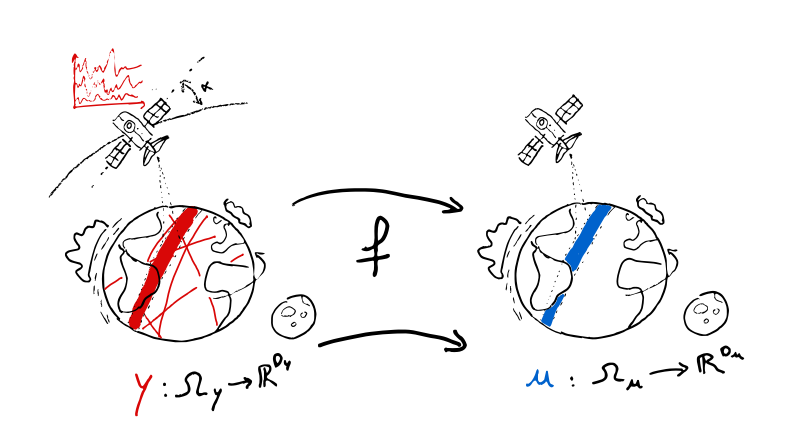
\includegraphics[width=\linewidth]{Introduction/pics/calib_task.png}    
      \caption{SWOT calibration problem. The left part illustrate the observed domain in red while the right part indicates the domain on which we aim at estimating the SSH.
      \label{fig:calibration_task}
  \end{figure}
The first observation problem we address is the estimation of sea surface height on the domain observed by the KaRIN instrument of the SWOT mission from scarce calibrated altimetry observations and uncalibrated SWOT observations.
As mentionned above, the KaRIN instrument deployed during the SWOT will contain both unprecedented errors and information about the sea surface height.
We are more precisely interested in the removal of correlated errors due to systematic instrument errors and noise-inducing geophysical processes.
The domain knowledge to design the model include theory about both the instrument physics as well as the SSH dynamics.

This use case also highlights the challenge when evaluating solution to observations problems, indeed we expect the SSH from the SWOT satellite to contain previously unobserved fine structures.
Therefore how can one evaluate the estimated fine structures in absence of reference data.
One way to address this, is to perform the evaluation through observing system simulation experiments by using simulated observations and SSH, but the question of representativeness of the simulated data with respect to operational settings needs to be considered carefully.
Another way to partially evaluate the calibration result is to confront the SSH with some altimetry data that has not been used for calibration.
Finally this is the point where domain expertise is invaluable, since in absence of precise quantification of the quality of the calibration, the qualitative assessment of likeliness and physical plausibility of the estimated field can represent a crucial guide.

For this task the operational approach consist in compiling assumptions about the processes and struture of the error signals and estimating the parameters of the sources of the errors.



\subsection{Altimetry Mapping}

  \begin{figure}
      \centering
            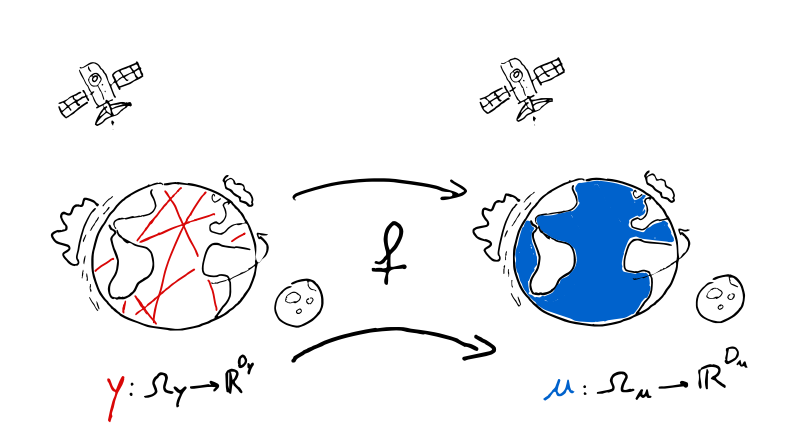
\includegraphics[width=\linewidth]{Introduction/pics/mapping_task.png}
      \caption{Nadir Altimetry problem. The left part illustrate the observed domain in red while the right part indicates the domain on which we aim at estimating the SSH.
      \label{fig:mapping_task}
  \end{figure}

The second observation problem we address is the estimation of sea surface height on daily maps from scarce calibrated altimetry observations. This can be viewed as an spatial and temporal interpolation of sparsely observed SSH to a dense domain.
Contrary to the KaRIN calibration which is a novel task, the mapping of NADIR altimeter task has been addressed by a variety of methods. Those methods use different assumptions and algorithm to estimate the maps of SSH.

% TO FILL: introduce different methods

\section{Deep learning potential for altimetry problems}

\subsection{Deep learning for computer vision and natural language processing}
Deep learning brings forth models, such as neural networks, that are predicated on very weak assumptions. Their strength lies in the fact that, given sufficient parameters, they can approximate any function\cite{}. This leads to deep learning models defining vast sets of potential candidates, consequently requiring substantial datasets and sophisticated algorithms to find the best fit.

Innovations in model architectures such as ResNet\cite{}, batch normalization\cite{}, and in optimization procedures\cite{} like Stochastic Gradient Descent (SGD)\cite{}, Adam\cite{}, and various learning rate schedules have consistently improved the search of larger spaces for candidate solutions, therefore  enabling the use of larger neural networks. 
However, the fact that deep learning models can in theory approximate any function introduces a peculiar consideration which is that fitting exactly the calibration data gives you no guarantee on how the model will behave on unseen data. The gap of performance between "seen" and "unseen" data is called the generalization gap. This has standardized the practice of splitting the calibration data in two sets: training and validation. The training set is used by the optimization procedure to search for the parameters whereas the validation set is used to assess the quality of each candidate. 
Addressing the problem of generalization have motivated many innovations in regularization, architectures, initialization schemes and data augmentation techniques.


When looking at different application domain, the track records of deep learning in computer vision\cite{} and natural language\cite{} are especially impressive. 
The combination of models and algorithm brought by deep learning have managed to solve tasks that previously unsolved.
This can be intuitively understood when considering the challenges of a binary classification task between cats and dogs.
Precisely that the mapping between natural images to binary label is quite difficult to explicitly formalize using domain knowledge. 
The task of predicting the next word of a sentence as done by current Large Language Models is similarly challenging to model using linguistic theory.

Presented as such deep learning seems to provide universal tools,  
however we would like to stress two factors that seem of great importance when looking at the contributions of deep learning in specific fields.
The first factor is quality and availability of data.
Indeed the creation of large, curated datasets, like ImageNet\cite{} in computer vision or ThePile\cite{} in natural language processing have shown to dramatically expedite the development of novel approaches. 
The second factor is the design of informed architectural patterns that are particularly suited to the domain, leading to performance breakthroughs. Examples of these include convolution techniques and U-Net architectures in computer vision, and attention mechanisms in natural language processing.


\subsection{Deep learning for altimetry}
Compared to other application domain such as computer vision and natural language processing, the altimetry problems present a different context for applying deep learning. 
On one hand quite extensive theoretical knowledge have been accumulated on the physical processes that give structure to the data and that explicitly links the observations with the quantities of interests.  
On the other hand the available data made of observations and numerical model outputs, although consequent, presents challenges since we never have access to the ground truth quantity we want to estimate. (The best we can do is consider a calibrated instrument as ground truth when available). 

This manuscript will specifically address these two facets — lack of ground truthed datasets and efficient architectural patterns — of deep learning when applied to observation exploitation.



Given a problem stated as above, deep learning brings to the table its set of tools for defining candidate solutions to a problem as well as optimization procedures for searching this set for the optimal candidate.
However the evaluation of 





This constitutes an interesting setup for synergizing physical priors and deep learning models.

Given the 


The scientific questions we raise can therefore be summarized as: Are the architectures and optimization introduced by deep learning suited for solving ocean altimetry problems ? How can domain specific knowledge about a specific problem inform the model used to address and observation problem? 




\subsection{Thesis outline}
More precisely we'll ask wether deep learning can help better exploit satellite observations for improving our knowledge of sea surface dynamics.


Deep learning and earth observation are two well established fields with accumulated knowledge, conventions, and best practices. 
This introduce challenges when developing transdisciplinary approaches that aim to combine expertise from the two fields.
Interfaces need to be proposed to this end which will serve as bridge for domain experts to explore the other side.
Evaluation and data from ocean scientists to ML practicioners. 
Didactic, Generic purpose, and modular implementation of a neural data assimation algorithm for addressing a range of observation problems from ML to ocean



\end{bibunit}

